%! Mode:: "TeX:UTF-8"
%! TEX program = xelatex
\PassOptionsToPackage{quiet}{xeCJK}
\documentclass[withoutpreface,bwprint]{cumcmthesis}
\usepackage{etoolbox}
\BeforeBeginEnvironment{tabular}{\zihao{-5}}
\usepackage[numbers,sort&compress]{natbib}  % 文献管理宏包
\usepackage[framemethod=TikZ]{mdframed}  % 框架宏包
\usepackage{url}  % 网页链接宏包
\usepackage{subcaption}  % 子图宏包
\newcolumntype{C}{>{\centering\arraybackslash}X}
\newcolumntype{R}{>{\raggedleft\arraybackslash}X}
\newcolumntype{L}{>{\raggedright\arraybackslash}X}

\title{全国大学生数学建模竞赛论文模板}  % 论文标题
\tihao{}  % 题号
\baominghao{}  % 报名号
\schoolname{}  % 学校
\membera{}  % 队员a
\memberb{}  % 队员b
\memberc{}  % 队员c
\supervisor{}  % 指导老师
\yearinput{}
\monthinput{}
\dayinput{}

%%%%%%%%%%%%%%%%%%%%%%%%%%%%%%%%%%%%%%%%%%%%%%%%%%%%%%%%%%%%%
%% 正文
\begin{document}

\maketitle
\begin{abstract}
摘要

\textbf{对于问题一,}

\textbf{对于问题二,}

\textbf{对于问题三,}

\textbf{对于问题四,}

最后,



\keywords{关键词\quad  关键词\quad  关键词\quad  关键词 \quad 关键词}
\end{abstract}
%%%%%%%%%%%%%%%%%%%%%%%%%%%%%%%%%%%%%%%%%%%%%%%%%%%%%%%%%%%%% 

% \tableofcontents  % 目录
% \newpage

%%%%%%%%%%%%%%%%%%%%%%%%%%%%%%%%%%%%%%%%%%%%%%%%%%%%%%%%%%%%%  
\section{问题重述}
\subsection{问题背景}
丝绸之路作为古代中西方文化交流的核心通道,玻璃是早期贸易往来的重要物证。
早期西亚和埃及的玻璃多以珠形饰品传入我国,我国古代吸收其技术后,
利用本土原料制作玻璃,虽外观与外来品相似,但因助熔剂差异(如铅矿石、草木灰等),
化学成分截然不同,形成了铅钡玻璃(我国自创,以楚文化为代表)、
高钾玻璃(流行于岭南及东南亚、印度等区域)等本土特色品种。
古代玻璃因埋藏环境易风化,风化过程中元素交换导致成分比例改变,
影响类别判断,而部分风化文物表面仍保留未风化区域,为成分研究提供了特殊样本,
对于研究古代中国社会和玻璃工艺具有很高的价值。

%%%%%%%%%%%%%%%%%%%%%%%%%%%%%%%%%%%%%%%%%%%%%%%%%%%%%%%%%%%%% 

\subsection{问题要求}

\textbf{问题1}  
分析玻璃文物的表面风化状态与其类型(高钾玻璃 / 铅钡玻璃)、
纹饰、颜色之间的关联;结合玻璃类型,
总结文物表面有无风化时化学成分含量的统计规律;
并基于风化点的检测数据,预测其风化前的化学成分含量。

\textbf{问题2}  
依据附件数据,提炼高钾玻璃与铅钡玻璃的分类规律;
针对这两类玻璃,分别选取合适的化学成分进行亚类划分,
明确具体的划分方法及结果,并分析该分类结果的合理性与敏感性。

\textbf{问题3} 
对附件表单 3 中未知类别的玻璃文物,通过分析其化学成分鉴别其所属类型
(高钾玻璃或铅钡玻璃),并对该分类结果的敏感性进行分析。

\textbf{问题4}  
针对高钾玻璃和铅钡玻璃这两类不同的文物样品,
分别分析其内部化学成分之间的关联关系,
并比较两类玻璃在化学成分关联关系上的差异性。
%%%%%%%%%%%%%%%%%%%%%%%%%%%%%%%%%%%%%%%%%%%%%%%%%%%%%%%%%%%%% 

\section{问题分析}
\subsection{问题一分析}
对于问题一,

\subsection{问题二分析}	
对于问题二,

\subsection{问题三分析}
对于问题三,

\subsection{问题四分析}
对于问题四,

%%%%%%%%%%%%%%%%%%%%%%%%%%%%%%%%%%%%%%%%%%%%%%%%%%%%%%%%%%%%% 

\section{模型假设}

为简化问题,本文做出以下假设:

\begin{itemize}[itemindent=2em]
\item 假设1
\item 假设2
\item 假设3
\end{itemize}

%%%%%%%%%%%%%%%%%%%%%%%%%%%%%%%%%%%%%%%%%%%%%%%%%%%%%%%%%%%%% 

\section{符号说明}
\begin{table}[H]
\centering
\begin{tabularx}{\textwidth}{CLC}
\toprule
符号    & 说明    & 单位 \\
\midrule
$m     $& 质量 & $kg$ \\
$V     $& 体积 & $m^3$ \\
\bottomrule
\end{tabularx}
\label{tab:符号说明}
\end{table}


%%%%%%%%%%%%%%%%%%%%%%%%%%%%%%%%%%%%%%%%%%%%%%%%%%%%%%%%%%%%% 

\section{问题一的模型的建立和求解}
\subsection{玻璃类型、颜色、纹饰与风化的关系}
首先我们对表单2中各文物采样点的化学成分进行累加,其中样本编号为15、17的文物
化学成分总和分别为79.47\%、71.89\%,不满足题目对成分比例累加和介于 
85\%~105\%之间的要求,因此我们将其剔除。

为了分析表面风化与玻璃类型、纹饰、颜色之间的关系,我们分别统计
(表面风化,玻璃类型)(表面风化,纹饰)(表面风化,颜色)这三个二元组
的列联表数据,并进行了可视化。

% 表1:表面风化与颜色的列联表(单独一行)
\begin{table}[htbp]
    \centering
    \caption{表面风化与颜色的列联表}
    \begin{tabular}{lcccccccc}
        \toprule
        \multirow{2}{*}{表面风化} & \multicolumn{8}{c}{颜色} \\
        \cmidrule(lr){2-9}
        & 浅绿 & 浅蓝 & 深绿 & 深蓝 & 紫 & 绿 & 蓝绿 & 黑 \\
        \midrule
        无风化 & 2 & 6 & 3 & 2 & 2 & 1 & 6 & 0 \\
        风化 & 1 & 12 & 4 & 0 & 2 & 0 & 9 & 2 \\
        \bottomrule
    \end{tabular}
\end{table}

% 表2和表3并排显示(同一行)
\begin{table}[htbp]
    \centering
    % 表2:表面风化与纹饰
    \begin{subtable}[t]{0.45\textwidth}
        \centering
        \caption{表面风化与纹饰的列联表}
        \begin{tabular}{lccc}
            \toprule
            \multirow{2}{*}{表面风化} & \multicolumn{3}{c}{纹饰} \\
            \cmidrule(lr){2-4}
            & A & B & C \\
            \midrule
            无风化 & 11 & 0 & 11 \\
            风化 & 11 & 6 & 17 \\
            \bottomrule
        \end{tabular}
    \end{subtable}
    \hspace{-15mm}% 两表之间的水平间距
    % 表3:表面风化与玻璃类型
    \begin{subtable}[t]{0.45\textwidth}
        \centering
        \caption{表面风化与玻璃类型的列联表}
        \begin{tabular}{lcc}
            \toprule
            \multirow{2}{*}{表面风化} & \multicolumn{2}{c}{类型} \\
            \cmidrule(lr){2-3}
            & 铅钡 & 高钾 \\
            \midrule
            无风化 & 12 & 10 \\
            风化 & 28 & 6 \\
            \bottomrule
        \end{tabular}
    \end{subtable}
    \caption{表面风化与纹饰、玻璃类型的列联表} % 总标题(可选)
\end{table}

\begin{figure}[ht]
\centering
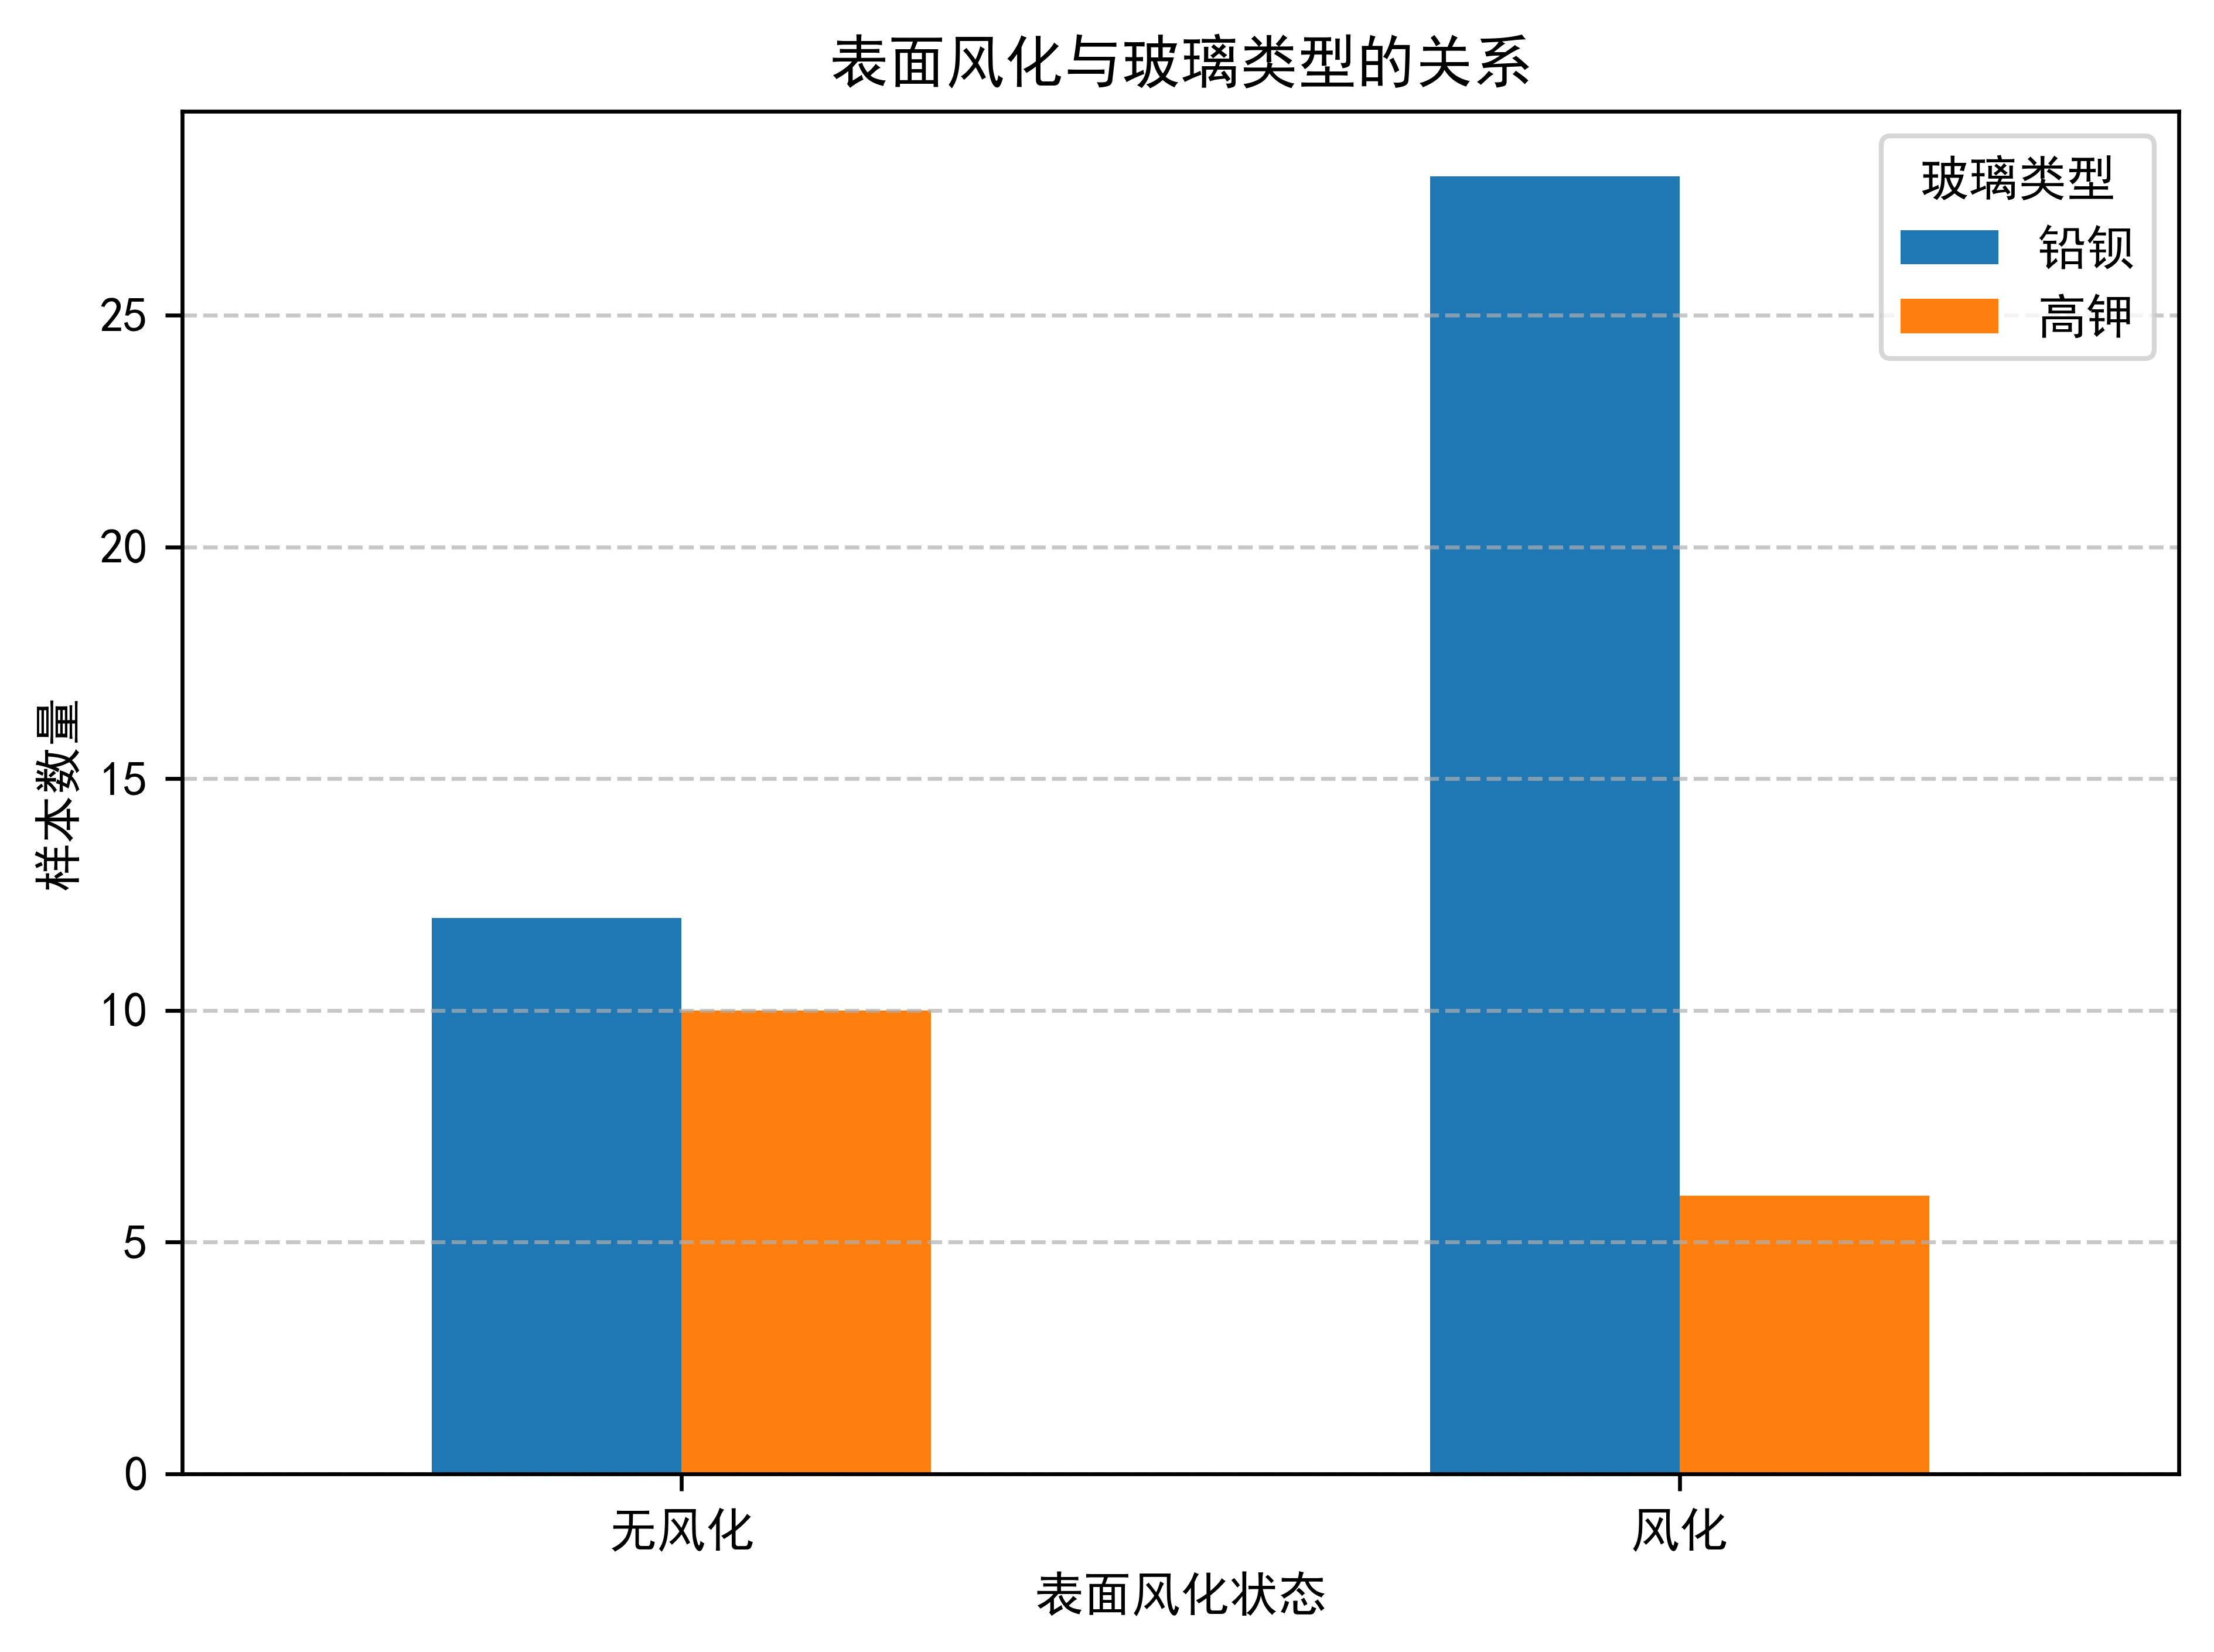
\includegraphics[width=0.6\textwidth]{figures/V4/1-1.png}
\caption{表面风化与玻璃类型}
\label{fig:表面风化与玻璃类型}
\end{figure}

\begin{figure}[ht]
\centering
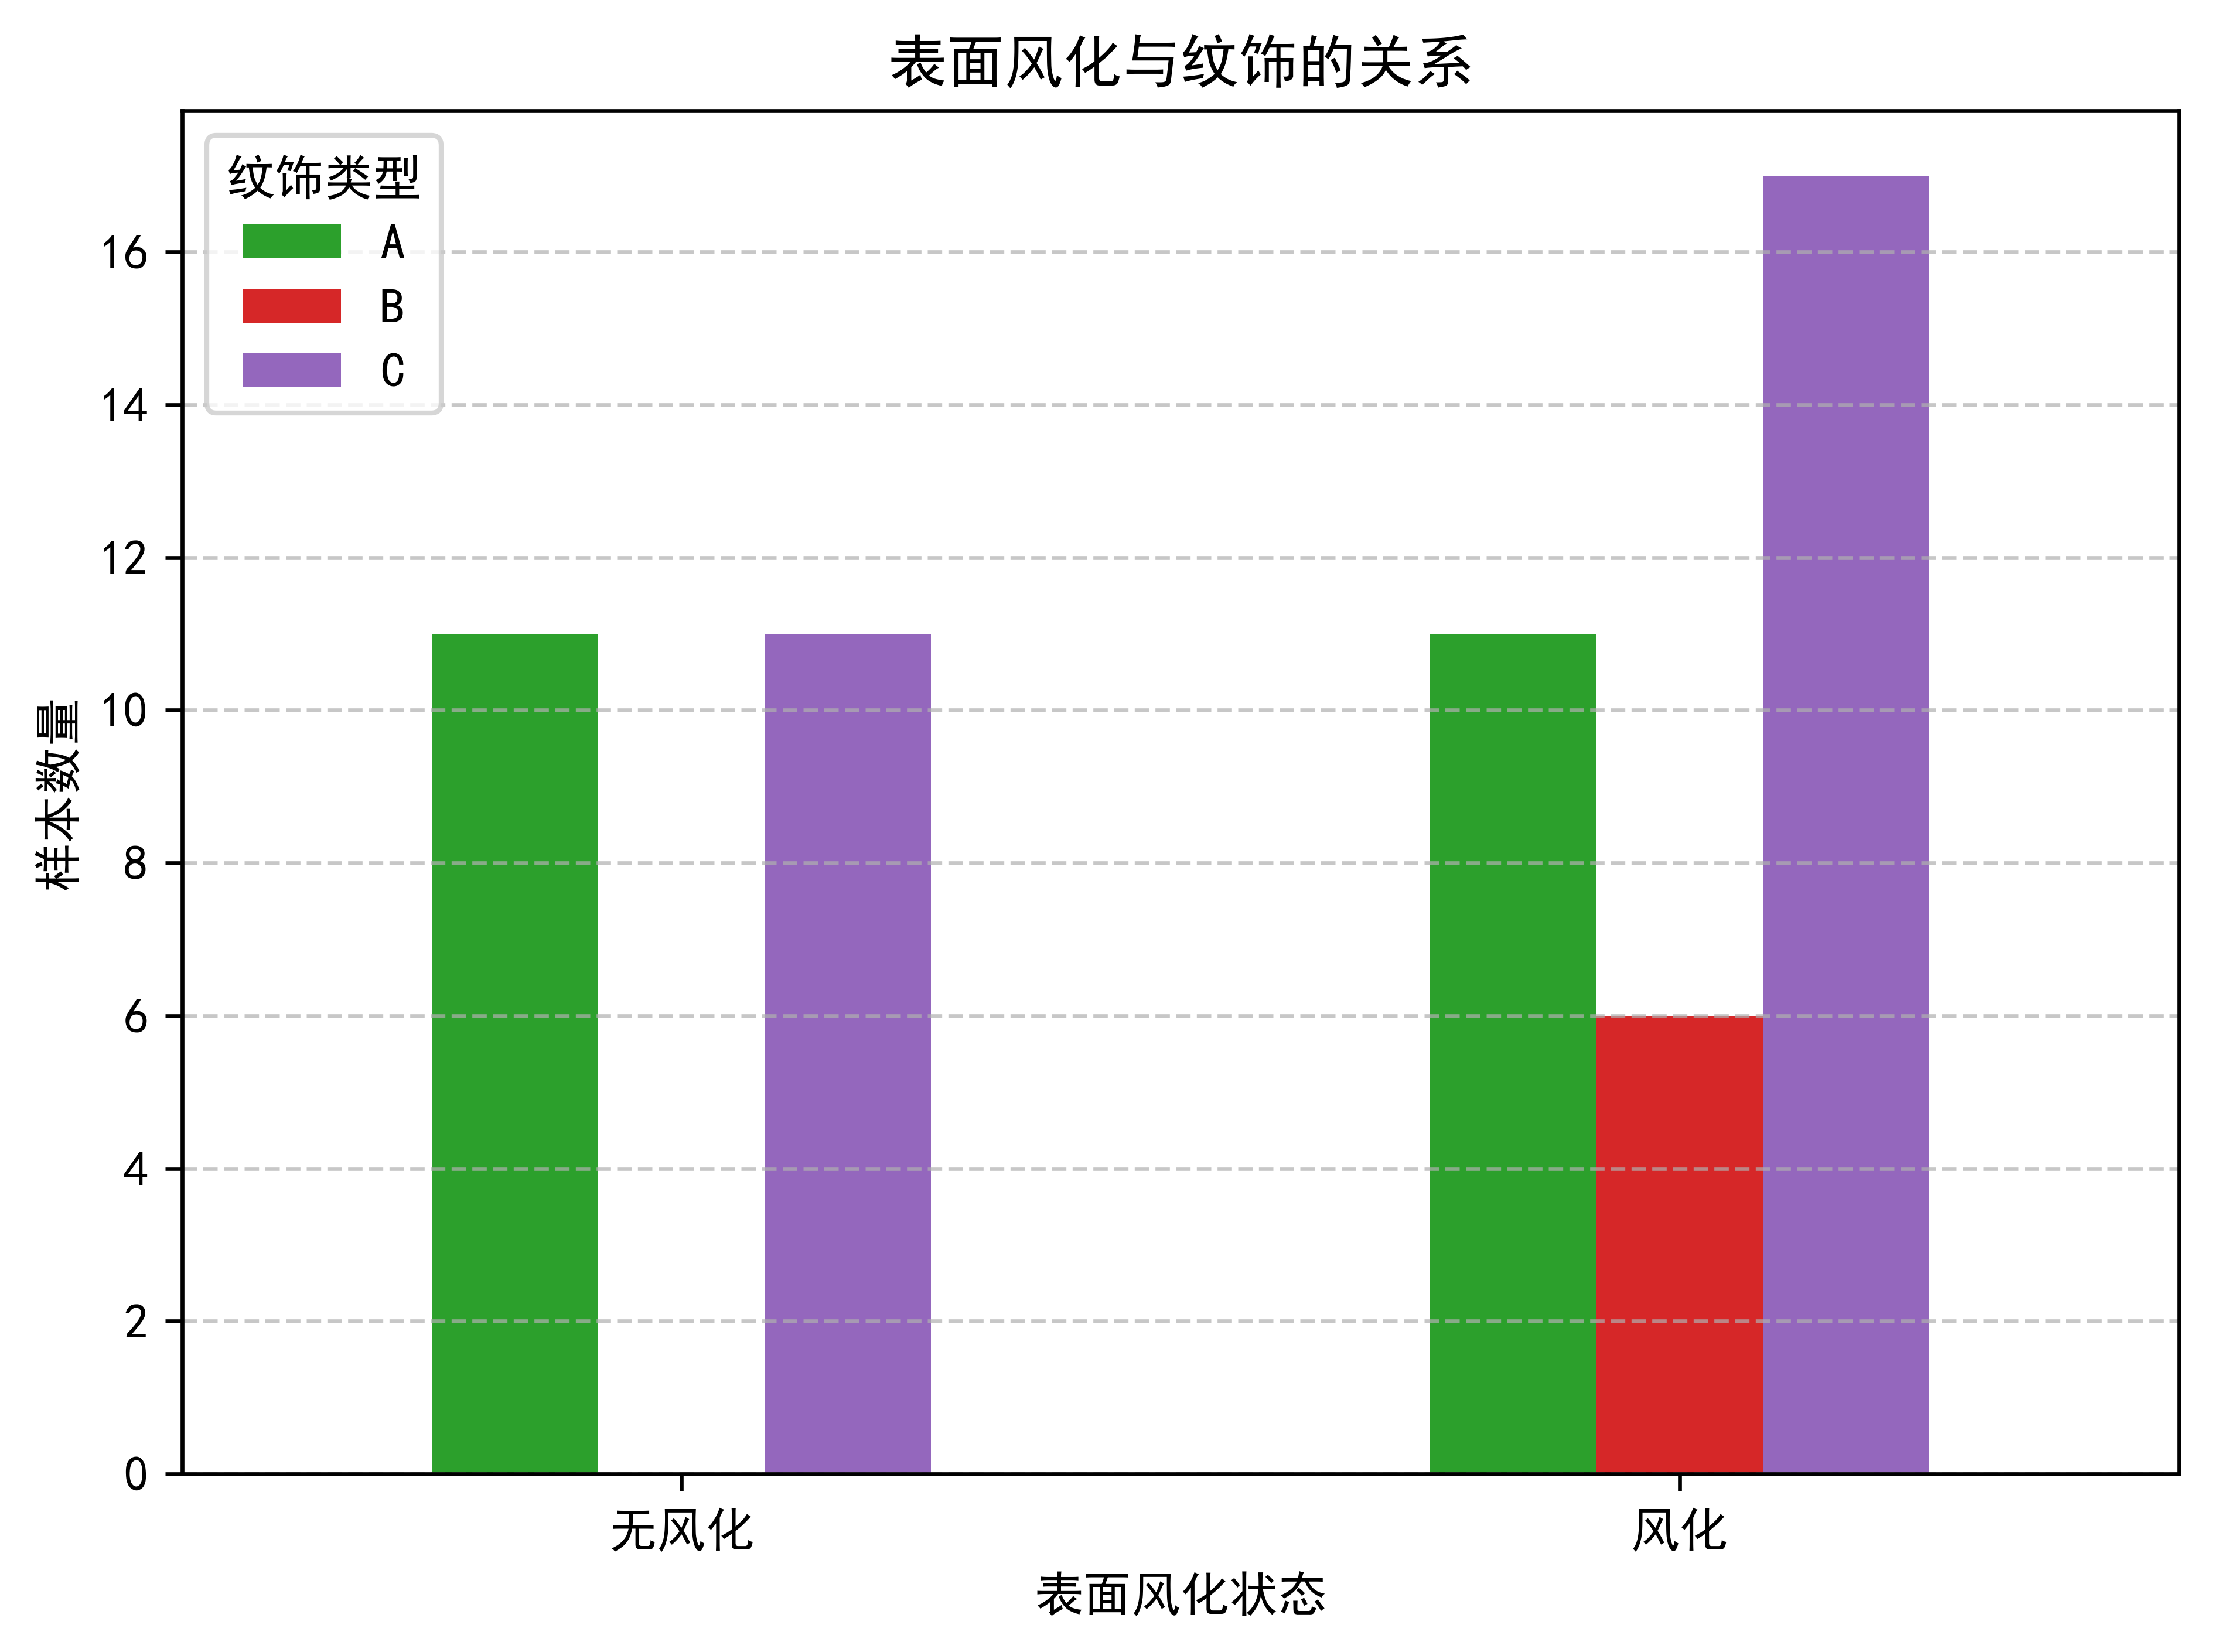
\includegraphics[width=0.6\textwidth]{figures/V4/1-2.png}
\caption{表面风化与纹饰}
\label{fig:表面风化与纹饰}
\end{figure}

\begin{figure}[ht]
\centering
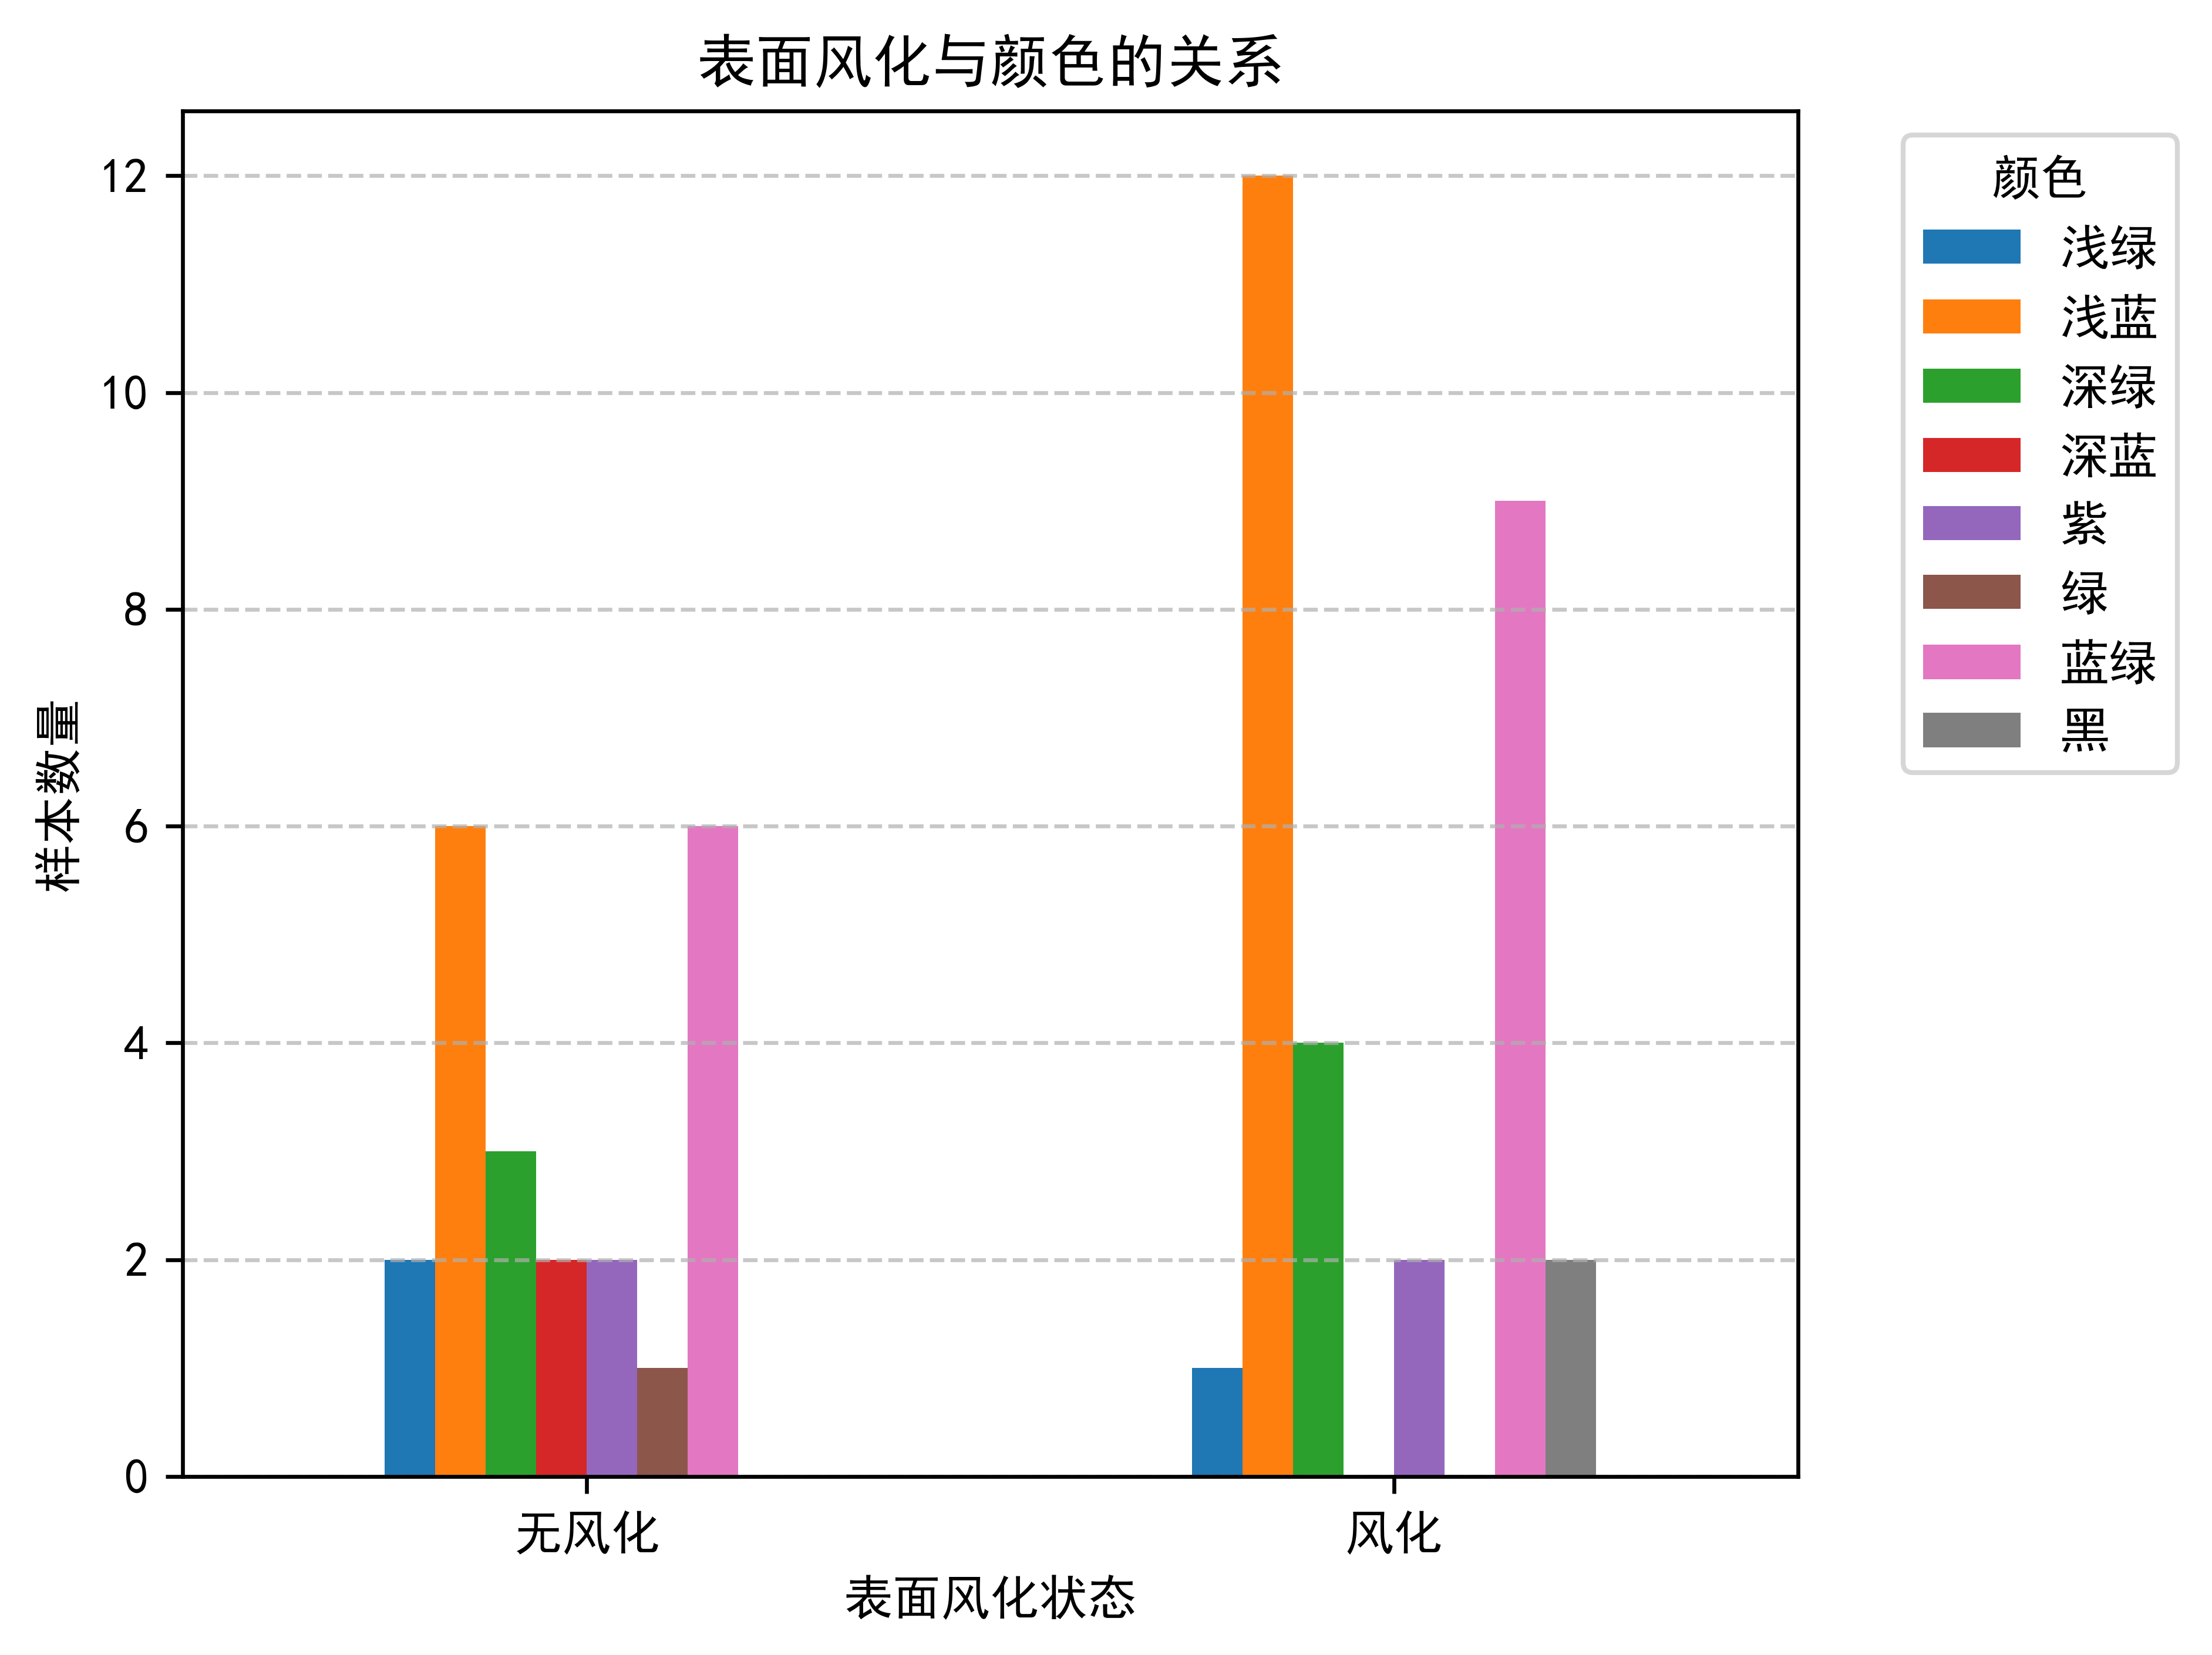
\includegraphics[width=0.6\textwidth]{figures/V4/1-3.png}
\caption{表面风化与颜色}
\label{fig:表面风化与颜色}
\end{figure}

为了量化表面风化与玻璃类型、纹饰、颜色之间的关系,我们引入了卡方检验。
卡方检验用于检验两个分类变量是否独立,通过比较观测值与期望值的差异,
用 $\chi^2$ 统计量判断关联是否显著,适用于计数数据。

%引用公式\cref{eq:公式1}。

\begin{equation}
\label{eq:公式1}
\chi^2 = \sum \frac{(O - E)^2}{E}
\end{equation}

其中:
 $\chi^2$:卡方统计量;
 $O$:实际观测频数;
 $E$:理论期望频数;
 $\sum$:对所有单元格求和。

分别带入(表面风化,玻璃类型)(表面风化,纹饰)(表面风化,颜色)的
列联表数据可以求出$\chi^2$值和$p$值,我们这里取$p<0.005$。从下面的表格中我们可以看出,
是否风化与玻璃类型之间存在显著关系,而风化与纹饰、颜色之间则不存在显著关系。

\begin{table}[htbp]
    \centering
    \caption{卡方检验结果}
    \begin{tabular}{lcccc}
        \toprule
        关系 & $\chi^2$ & $df$ & $p$值 &  是否显著 \\
        \midrule
        风化 $\times$ 颜色 & 7.0114 & $(2-1)\times(8-1)=7$ & $p \approx 0.426$ & 否 \\
        风化 $\times$ 纹饰 & 4.9412 & $(2-1)\times(3-1)=2$ & $p \approx 0.085$ & 否 \\
        风化 $\times$ 类型 & 5.0610 & $(2-1)\times(2-1)=1$ & $p \approx 0.024$ & 是 \\
        \bottomrule
    \end{tabular}
\end{table}

\subsection{玻璃是否风化化学成分含量的统计规律}

以文物采样点为单位,以玻璃类型、是否风化为分组依据,
我们统计了每种组别的化学成分含量。


%引用\cref{fig:单图}。

\begin{figure}[ht]
\centering
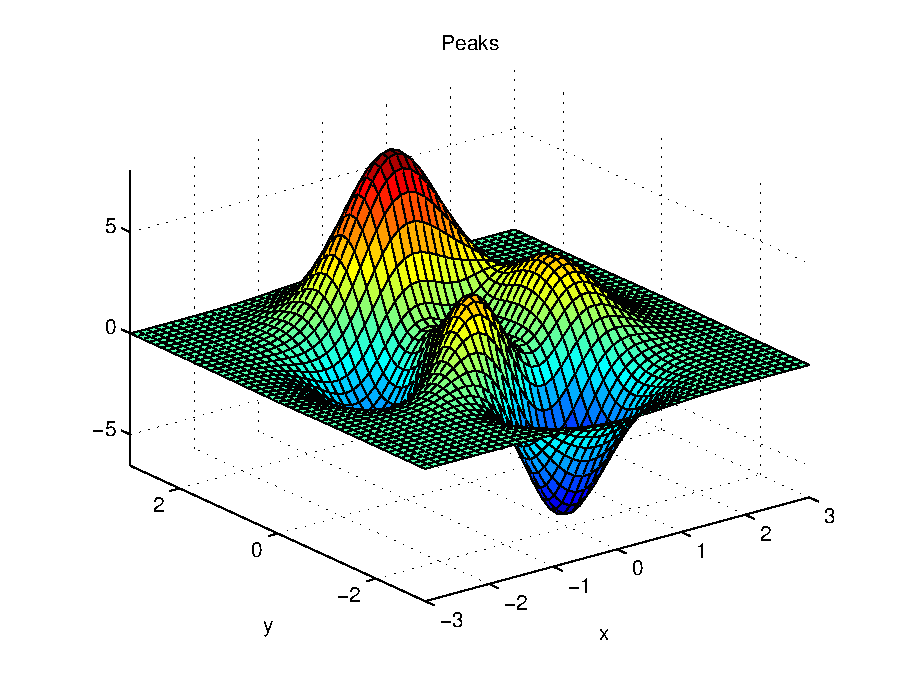
\includegraphics[width=0.75\textwidth]{example.eps}
\caption{单图}
\label{fig:单图}
\end{figure}

这句话引用了文献\cite{司守奎2011数学建模算法与应用}。

这句话引用了文献\upcite{卓金武2011MATLAB}。

\subsection{模型求解}

\textbf{Step1:} 

\textbf{Step2:} 

\textbf{Step3:} 

\subsection{求解结果}


%%%%%%%%%%%%%%%%%%%%%%%%%%%%%%%%%%%%%%%%%%%%%%%%%%%%%%%%%%%%% 

\section{问题二的模型的建立和求解}
\subsection{模型建立}

引用\cref{fig:双图},引用\cref{fig:双图a},引用\cref{fig:双图b}。

\begin{figure}[ht]
\centering
\subcaptionbox{双图a子标题\label{fig:双图a}}
{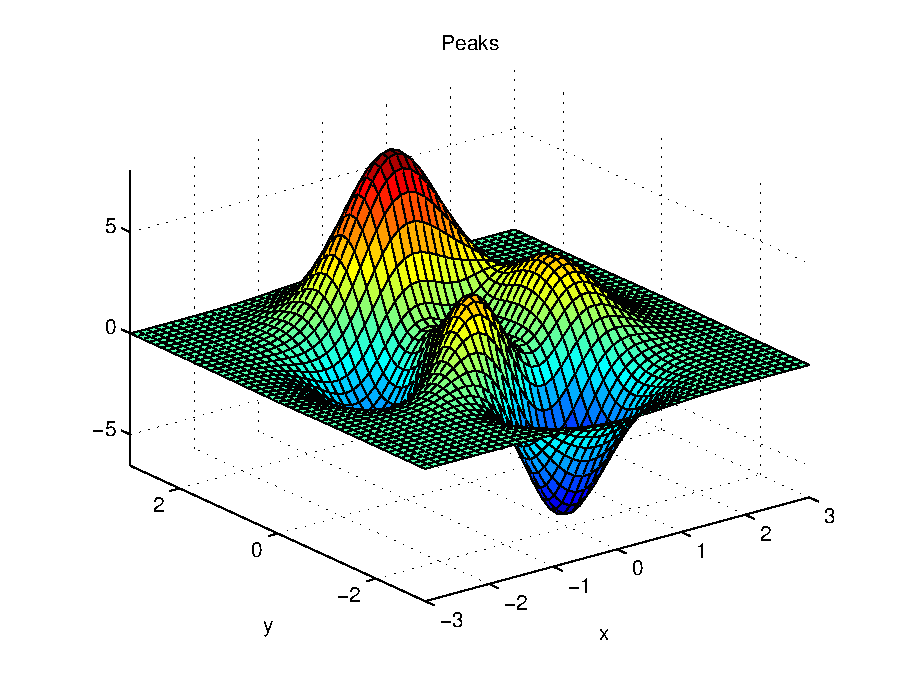
\includegraphics[width=.4\textwidth]{example.eps}}
\subcaptionbox{双图b子标题\label{fig:双图b}}
{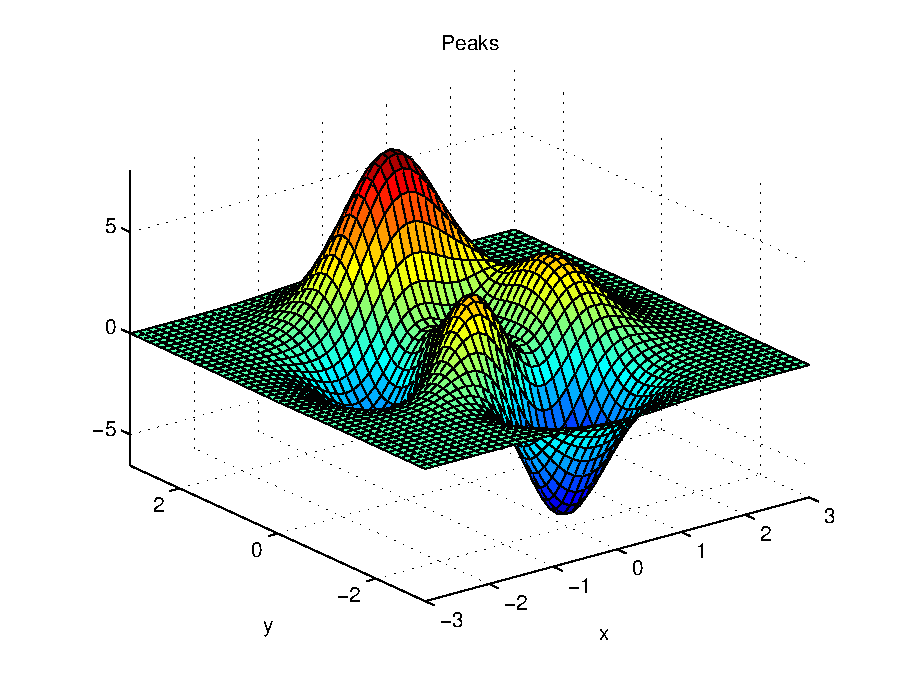
\includegraphics[width=.4\textwidth]{example.eps}}
\caption{双图}\label{fig:双图}
\end{figure} 

\subsection{模型求解}

\textbf{Step1:} 

\textbf{Step2:} 

\textbf{Step3:} 

\subsection{求解结果}

%%%%%%%%%%%%%%%%%%%%%%%%%%%%%%%%%%%%%%%%%%%%%%%%%%%%%%%%%%%%% 

\section{问题三的模型的建立和求解}
\subsection{模型建立}

\subsection{模型求解}

\textbf{Step1:} 

\textbf{Step2:} 

\textbf{Step3:} 

\subsection{求解结果}

%%%%%%%%%%%%%%%%%%%%%%%%%%%%%%%%%%%%%%%%%%%%%%%%%%%%%%%%%%%%% 

\section{问题四的模型的建立和求解}
\subsection{模型建立}

\subsection{模型求解}

\textbf{Step1:} 

\textbf{Step2:} 

\textbf{Step3:} 

\subsection{求解结果}

%%%%%%%%%%%%%%%%%%%%%%%%%%%%%%%%%%%%%%%%%%%%%%%%%%%%%%%%%%%%%

\section{模型的分析与检验}

\subsection{灵敏度分析}

\subsection{误差分析}

%%%%%%%%%%%%%%%%%%%%%%%%%%%%%%%%%%%%%%%%%%%%%%%%%%%%%%%%%%%%%

\section{模型的评价}

\subsection{模型的优点}
\begin{itemize}[itemindent=2em]
\item 优点1
\item 优点2
\item 优点3
\end{itemize}

\subsection{模型的缺点}
\begin{itemize}[itemindent=2em]
\item 缺点1
\item 缺点2
\end{itemize}

%%%%%%%%%%%%%%%%%%%%%%%%%%%%%%%%%%%%%%%%%%%%%%%%%%%%%%%%%%%%%
%% 参考文献
\nocite{*}
\bibliographystyle{gbt7714-numerical}  % 引用格式
\bibliography{ref.bib}  % bib源

\newpage
%%%%%%%%%%%%%%%%%%%%%%%%%%%%%%%%%%%%%%%%%%%%%%%%%%%%%%%%%%%%%
%% 附录
\begin{appendices}
\section{文件列表}
\begin{table}[H]
\centering
\begin{tabularx}{\textwidth}{LL}
\toprule
文件名   & 功能描述 \\
\midrule
q1.m & 问题一程序代码 \\
q2.py & 问题二程序代码 \\
q3.c & 问题三程序代码 \\
q4.cpp & 问题四程序代码 \\
\bottomrule
\end{tabularx}
\label{tab:文件列表}
\end{table}

\section{代码}
\noindent q1.m
\lstinputlisting[language=matlab]{code/q1.m}
q2.py
\lstinputlisting[language=python]{code/q2.py}
q3.c
\lstinputlisting[language=c]{code/q3.c}
q4.cpp
\lstinputlisting[language=c++]{code/q4.cpp}
\end{appendices}
\end{document}


%%%%%双图模板%%%%%%
\begin{figure}
\centering
\subcaptionbox{炉温曲线示意图\label{fig:双图a}}
{\includegraphics[width=.4\textwidth]{炉温曲线示意图.png}}
\subcaptionbox{问题1炉温曲线\label{fig:双图b}}
{\includegraphics[width=.4\textwidth]{问题1炉温曲线.png}}
\caption{双图}\label{fig:双图}
\end{figure} 
%%%%%双图模板%%%%%%